
\documentclass{article}
\usepackage{url,graphicx,tabularx,array,geometry, hyperref}
\usepackage{listings}
\usepackage{fullpage}
\usepackage{fancyvrb}
\usepackage{framed}
\usepackage{lastpage}
\usepackage{fancyhdr}
\usepackage{float}

\renewcommand{\headrulewidth}{0pt}
\setcounter{secnumdepth}{0}

\setlength{\parskip}{1ex} %--skip lines between paragraphs
\setlength{\parindent}{0pt} %--don't indent paragraphs
\setlength{\headheight}{15.2pt}

\pagestyle{fancy}

\renewcommand{\headrulewidth}{0pt}
\lhead{  }
\lfoot{Lab 1: TCP Congestion Control}
\rfoot{page \thepage\ of \pageref{LastPage}}

\renewcommand{\familydefault}{\sfdefault}
\begin{document}

\begin{titlepage}
\begin{center}
\textsc{\huge \bfseries Advanced Networking 2018}\\[1.5cm]
\textsc{\large Lab \#1: TCP Congestion Control}\\[1.5cm]
\textsc{\huge Report}\\[1.5cm]
\textsc{\huge \bfseries GROUP: 3}\\[1.5cm]
\textsc{\large{\textbf{Authors:}\\ 
Kotaiba Alachkar, Kotaiba.Alachkar@os3.nl\\ Andrey Afanas'yev, Andrey.Afanasyev@os3.nl\\
Rick van Gorp, Rick.Vangorp@os3.nl\\
Henri Trenquier, Henri.Trenquier@os3.nl
}}

\textsc{\large University of Amsterdam}
\end{center}
\end{titlepage}
\subsection{Q0.0 Preparation}

\textsc{\large Configuration of the switch:}

We used \textit{Calais} to connect to the \textit{Mgmt} network.
From there, we configured \textit{Calais} to connect the Switch \textit{Chico3}:

\begin{verbatim}
    ## AN lab2 ##
auto eno2
iface eno2 inet static
        address 10.0.1.203 #mgmt
        netmask 255.255.255.0
        broadcast 255.255.255.255
\end{verbatim}

After restarting the network service, we can connect to \textit{10.0.1.4} via ssh.
From the switch, we can access the second port with
\begin{verbatim}
    dialout@serialserv4:~ $ minicom -b 9600 -D /dev/ttyUSB1
\end{verbatim}

We can now configure the switch:
\begin{verbatim}
 !
 no service password-encryption
 !
 ip domain-name gr3.com
 !
 hostname gr3switch
 !
 interface Vlan1
 ip address 192.168.0.253 255.255.255.0
 !
 interface Loopback1
 no ip address
 !
 username andrey password 0 cisco
 username kotaiba password 0 cisco
 username rick password 0 cisco
 username henrilarose password 0 cisco
 !
 line con 0
 logging synchronous
 login local
line vty 0 4
 password 7cisco
 login local
 transport input ssh
line vty 5 15
 login
 !
\end{verbatim}

\textsc{\large Connection to the network:}

Later, we can disconnect the UTP connection to the \textit{Mgmt} and connect to \textit{gr3switch}.

The new interface configuration is:
\begin{verbatim}
    ## AN lab2 ##
auto eno2
iface eno2 inet static
        address 192.168.0.127
        netmask 255.255.255.0
        broadcast 255.255.255.255
\end{verbatim}

If we encounter this error:
\begin{verbatim}
    RTNETLINK answers: File exists 
    Failed to bring up eno2
\end{verbatim}

The following command has to be entered:
\begin{verbatim}
    sudo ip addr flush dev eno2
\end{verbatim}

Finally, it is possible to connect to the local network. We can ping every team member from Henri's server.:
Ping Rick:
\begin{verbatim}
    ~ \$ ping 192.168.0.200
PING 192.168.0.200 (192.168.0.200) 56(84) bytes of data.
64 bytes from 192.168.0.200: icmp_seq=1 ttl=64 time=0.391 ms
64 bytes from 192.168.0.200: icmp_seq=2 ttl=64 time=0.181 ms
^C
--- 192.168.0.200 ping statistics ---
2 packets transmitted, 2 received, 0% packet loss, time 999ms
rtt min/avg/max/mdev = 0.181/0.286/0.391/0.105 ms
\end{verbatim}
Ping Kotaiba:
\begin{verbatim}
    ~ \$ ping 192.168.0.69
PING 192.168.0.69 (192.168.0.69) 56(84) bytes of data.
64 bytes from 192.168.0.69: icmp_seq=1 ttl=64 time=0.295 ms
64 bytes from 192.168.0.69: icmp_seq=2 ttl=64 time=0.150 ms
^C
--- 192.168.0.69 ping statistics ---
2 packets transmitted, 2 received, 0% packet loss, time 999ms
rtt min/avg/max/mdev = 0.150/0.222/0.295/0.074 ms
\end{verbatim}
Ping Andrey:
\begin{verbatim}
    ~ \$ ping 192.168.0.3
PING 192.168.0.3 (192.168.0.3) 56(84) bytes of data.
64 bytes from 192.168.0.3: icmp_seq=1 ttl=64 time=0.205 ms
64 bytes from 192.168.0.3: icmp_seq=2 ttl=64 time=0.083 ms
^C
--- 192.168.0.3 ping statistics ---
2 packets transmitted, 2 received, 0% packet loss, time 999ms
rtt min/avg/max/mdev = 0.083/0.144/0.205/0.061 ms
\end{verbatim}
Ping the switch:
\begin{verbatim}
    ~ \$ ping 192.168.0.253
PING 192.168.0.253 (192.168.0.253) 56(84) bytes of data.
64 bytes from 192.168.0.253: icmp_seq=2 ttl=255 time=1.78 ms
^C
--- 192.168.0.253 ping statistics ---
2 packets transmitted, 1 received, 50% packet loss, time 999ms
rtt min/avg/max/mdev = 1.783/1.783/1.783/0.000 ms
\end{verbatim}


Finally, we can connect via ssh with the following command:
\begin{verbatim}
~ \$ ssh -o KexAlgorithms=diffie-hellman-group1-sha1  henri@192.168.0.253    
\end{verbatim}

Indeed, the switch's configuration doesn't allow more recent Key exchange algorithm.

To disable HTTP and HTTPS we use the following commands:
\begin{verbatim}
gr3switch(config)#no ip http server
gr3switch(config)#no ip http secure-server
\end{verbatim}


To disable Telnet on other Virtual Terminal lines:
\begin{verbatim}
gr3switch(config)#line vty 5 15
gr3switch(config-line)#transport input none
\end{verbatim}

\subsection{Q2.1 Data transfer without and with CoS configuration}
In this question we have used \textit{iperf} to transfer data between 192.168.0.69 and 192.168.0.200. The server has been set up using \texttt{iperf -s} and the client connected to the server using \texttt{iperf -c -u 192.168.0.69} and \texttt{iperf -c 192.168.0.69}. We have not selected a specific congestion algorithm as the switch is a Gigabit-switch, which matches the speed of the NICs of the servers. The throughput achieved is listed in \textit{Figure \ref{fig:throughput_iperf}} and \textit{Figure \ref{fig:throughput_iperf2}}. We have also tested using different requested window sizes: 100, 100.000 and 100.000.000 bytes. This did not improve the speed, compared to \texttt{iperf's} defaults.

\bigskip

\begin{figure}[h]
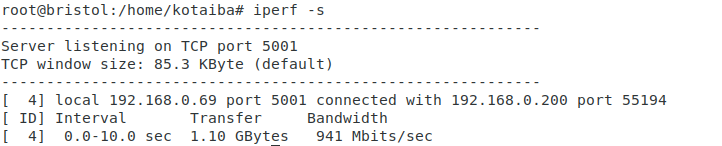
\includegraphics[width=8cm]{figures/q2-1-1.png}
\centering
\caption{TCP Performance}
\centering
\label{fig:throughput_iperf}
\end{figure}



\bigskip

\begin{figure}[h]
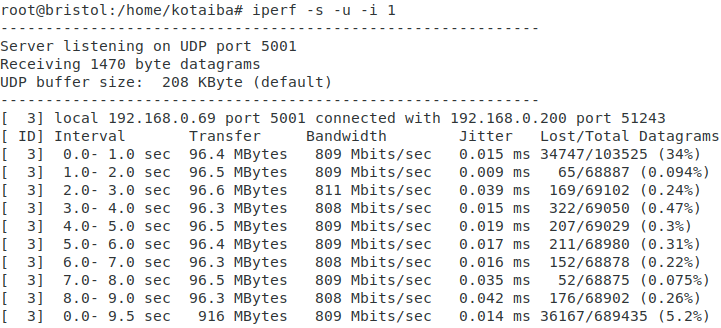
\includegraphics[width=8cm]{figures/q2-1-2.png}
\centering
\caption{UDP Performance}
\centering
\label{fig:throughput_iperf2}
\end{figure}


When we change the size of the MTU on interface \texttt{eno2}, the throughput decreases. This was done by configuring the MTU-size of the interface:
\begin{verbatim}
    ifconfig eno2 down
    ifconfig eno2 mtu 1000 up
\end{verbatim}

Then running the server and client with the -M option at 1000. Also when we decrease it to 100, the throughput decreases drastically.

\bigskip

\subsection{Q2.2 Define a number of scenarios where the data transfers interfere with each other}
After some discussion we could define following affordable scenarios, which simulate different computer network traffic:

\begin{enumerate}
    \item Example from lab one basic scenario could be the one in which multiple nodes and applications are trying to  communicate  with  one  node.
        \begin{itemize}
            \item Server node required to run two \textit{iperf} servers accepting the TCP and UDP traffic. Other two nodes generates TCP and UDP traffic respectively.
        \end{itemize}
    \item A single node communicates with another node while the rest two try to ping first host at higher time frequency and with large packet sizes (DDOS).
        \begin{itemize}
            \item Two nodes communicate using iperf running on TCP (server and client).
            \item The rest two have a ping a iperf server with the same ping configuration like: \texttt{ping -i 0.01 -s 65507 192.168.0.200}
        \end{itemize}    
    \item One node has a HTTP/1.1 server on board which stress tested by other two nodes another node communicates with first one via \texttt{iperf}.
    \begin{itemize}
        \item One server is configured with Nginx and HTTP/1.1 it has also iperf server on board
        \item Two nodes try to stress test Nginx using simple ab test like \textitt{ab -n 1000000 -c 100 http://192.168.0.200/}
        \item Last one node is an iperf client.
    \end{itemize}
\end{enumerate}

\subsubsection{Execution of the first scenario}
We have set up the first scenario by setting up two \texttt{iperf} listeners (UDP and TCP) on server \texttt{192.168.0.200}, using commands \texttt{iperf -s} for TCP and \texttt{iperf -s -p 5000 -u} for UDP. The clients then connected to the server's listeners using commands \texttt{iperf -c 192.168.0.200} and \texttt{iperf -c 192.168.0.200 -p 5000 -u -b 1200M}. The results of this test for the clients are shown in \textit{Figure \ref{fig:throughput_udp_test_1}, \ref{fig:throughput_tcp_test_1}, \ref{fig:throughput_udp_test_2} and \ref{fig:throughput_tcp_test_2}}. The results of this test for the server are shown in \textit{Figure \ref{fig:throughput_udp_result} and \ref{fig:throughput_tcp_result}}.

\begin{figure}[H]
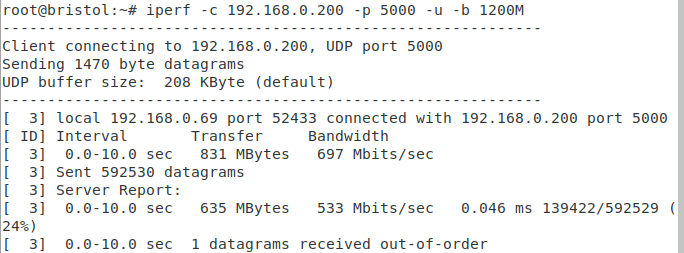
\includegraphics[width=14cm]{figures/q2-2-1-udp-1.png}
\centering
\caption{Scenario 1 - UDP Test 1}
\centering
\label{fig:throughput_udp_test_1}
\end{figure}


\begin{figure}[H]
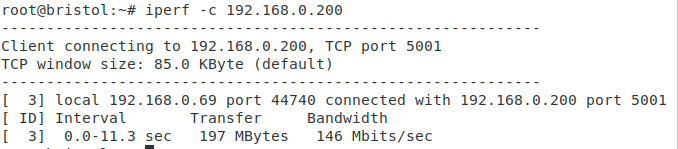
\includegraphics[width=14cm]{figures/q2-2-1-tcp-1.png}
\centering
\caption{Scenario 1 - TCP Test 1}
\centering
\label{fig:throughput_tcp_test_1}
\end{figure}


\begin{figure}[H]
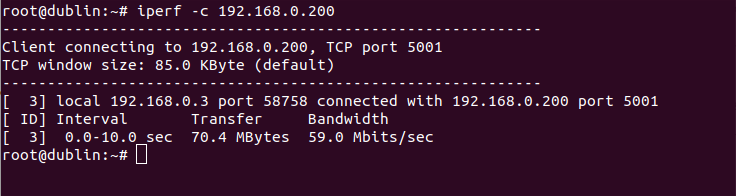
\includegraphics[width=14cm]{figures/q2-2-1-udp-2.png}
\centering
\caption{Scenario 1 - UDP Test 2}
\centering
\label{fig:throughput_udp_test_2}
\end{figure}


\begin{figure}[H]
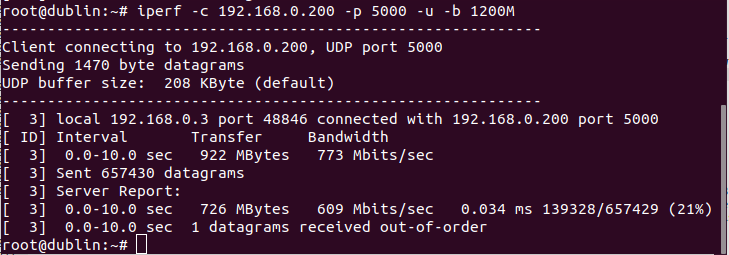
\includegraphics[width=14cm]{figures/q2-2-1-tcp-2.png}
\centering
\caption{Scenario 1 - TCP Test 2}
\centering
\label{fig:throughput_tcp_test_2}
\end{figure}


\begin{figure}[H]
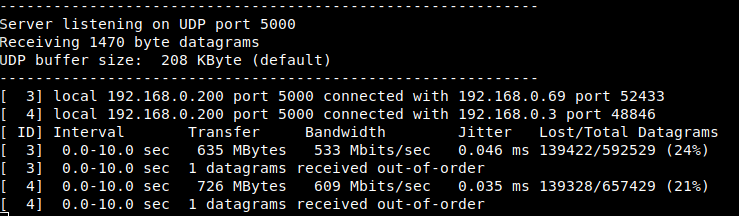
\includegraphics[width=14cm]{figures/q2-2-1-udp-result.png}
\centering
\caption{Scenario 1 - UDP Test result}
\centering
\label{fig:throughput_udp_result}
\end{figure}


\begin{figure}[H]
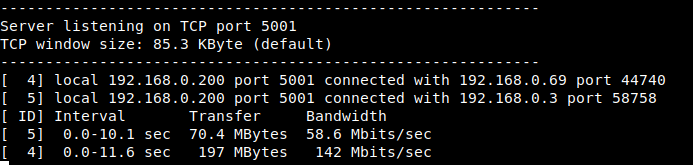
\includegraphics[width=14cm]{figures/q2-2-1-tcp-result.png}
\centering
\caption{Scenario 1 - TCP Test result}
\centering
\label{fig:throughput_tcp_result}
\end{figure}

From the results we can derive that there are different results for UDP and TCP traffic. According to \textit{Figure \ref{fig:throughput_udp_result} and \ref{fig:throughput_tcp_result}} the UDP traffic claims more bandwidth than the TCP traffic, resulting in the TCP traffic being pushed away. This can be (partially) solved using prioritisation of traffic.

\subsubsection{Execution of the second scenario}
In the second scenario we have set up an \texttt{iperf} server on \texttt{192.168.0.200}. We started a transfer on TCP towards the server in \texttt{iperf} from one client using \texttt{iperf -c 192.168.0.200}. At the same time, another pair of clients start a ping with large packet sizes using command \texttt{ping 192.168.0.200 -i 0.01 -s 65507}. The results for the \texttt{iperf} client are shown in \textit{Figure \ref{fig:throughput_scenario_2}}. The results of the ping clients are shown in \textit{Figures \ref{fig:throughput_scenario_2_ping_1} and \ref{fig:throughput_scenario_2_ping_2}}. The results of the \texttt{iperf} server is shown in \textit{Figure \ref{fig:throughput_scenario_2_result}}. 

\begin{figure}[H]
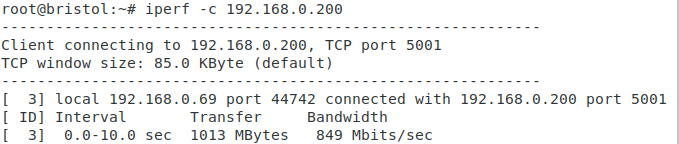
\includegraphics[width=14cm]{figures/q2-2-2-1.png}
\centering
\caption{Scenario 2 - TCP Iperf}
\centering
\label{fig:throughput_scenario_2}
\end{figure}

\begin{figure}[H]
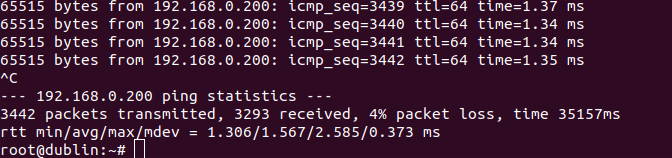
\includegraphics[width=14cm]{figures/q2-2-2-ping-2.png}
\centering
\caption{Scenario 2 - Large packet 1}
\centering
\label{fig:throughput_scenario_2_ping_1}
\end{figure}

\begin{figure}[H]
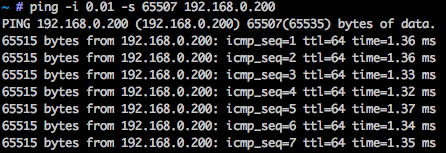
\includegraphics[width=14cm]{figures/q2-2-2-ping-1.png}
\centering
\caption{Scenario 2 - Large packet 2}
\centering
\label{fig:throughput_scenario_2_ping_2}
\end{figure}


\begin{figure}[H]
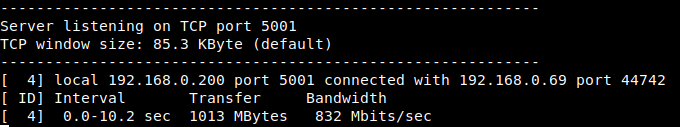
\includegraphics[width=14cm]{figures/q2-2-2-result.png}
\centering
\caption{Scenario 2 - Result}
\centering
\label{fig:throughput_scenario_2_result}
\end{figure}

In \textit{Figure \ref{fig:throughput_iperf}} we have shown the normal throughput for TCP-traffic between an \texttt{iperf} server and client. Because of the ping request sending large sized packets with a high frequency, approximately 110 Mbits/sec was allocated to the ICMP-traffic.


\subsubsection{Execution of the third scenario}
The third scenario will include an \texttt{Apache} webserver along with an \texttt{iperf} server both running on \texttt{192.168.0.200}. One client will communicate with the server using \texttt{iperf -c 192.168.0.200} and other two nodes will use a benchmarking tool like apache benchmark (ab) with the following command \texttt{b -n 100000 -c 10 http://192.168.0.200}. The results of the \texttt{iperf} client are shown in \textit{Figure \ref{fig:throughput_scenario_3}}. The results of the Apache benchmark clients are shown in \textit{Figures \ref{fig:ab_dublin_scenario_3} and \ref{fig:ab_calais_scenario_3}}. The results of the server are shown in \textit{Figure \ref{fig:throughput_scenario_3_result}}.


\begin{figure}[H]
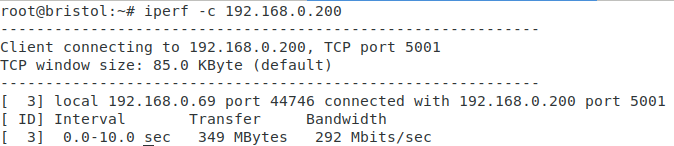
\includegraphics[width=14cm]{figures/q-2-2-3-1.png}
\centering
\caption{Scenario 2 - TCP Iperf}
\centering
\label{fig:throughput_scenario_3}
\end{figure}


\begin{figure}[H]
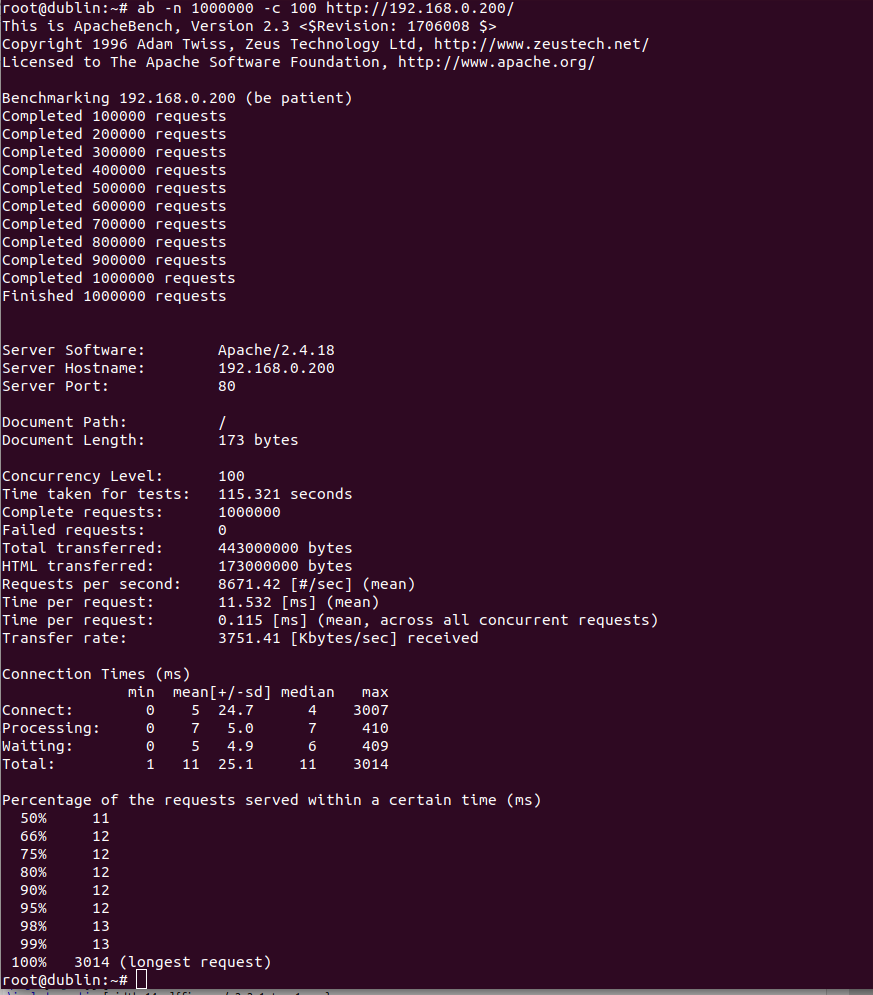
\includegraphics[width=14cm]{figures/dublin-ab.png}
\centering
\caption{Scenario 3 - Apache Benchmark from Dublin client server to Apache server}
\centering
\label{fig:ab_dublin_scenario_3}
\end{figure}

\begin{figure}[H]
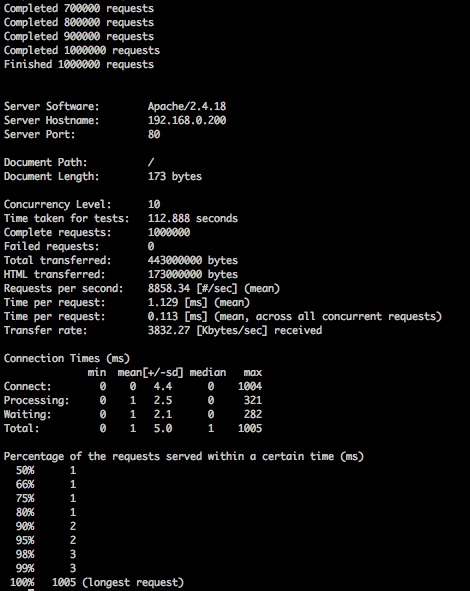
\includegraphics[width=14cm]{figures/calais-ab.png}
\centering
\caption{Scenario 3 - Apache Benchmark from client server to Apache server}
\centering
\label{fig:ab_calais_scenario_3}
\end{figure}


\begin{figure}[H]
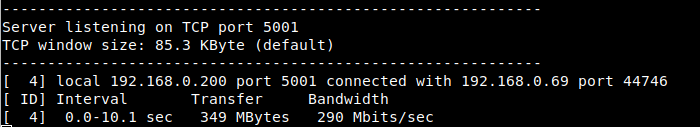
\includegraphics[width=14cm]{figures/q-2-2-3-results.png}
\centering
\caption{Scenario 2 - Result}
\centering
\label{fig:throughput_scenario_3_result}
\end{figure}

From these results we can derive the Apache Benchmark traffic's bandwidth allocation is much higher than the allocation of traffic to the \texttt{iperf} transfer. Again, this can be regulated by giving HTTP-traffic a lower priority than \texttt{iperf} traffic.

\subsection{Q3 Configuring CoS}
In order to configure CoS, it has to be enabled on the interfaces of the switch where the servers are connected to. First CoS has to be enabled globally on the switch by performing the following configuration steps on the switch:
\begin{verbatim}
    conf t
    mls qos
\end{verbatim}

We will prioritize two interfaces distributing the interfering traffic (Apache Benchmark) with a lower priority than the other interfaces. This is done by performing the following configuration steps on the switch:
\begin{verbatim}
    conf t
    int G1/0/17
    mls qos cos 6
    mls qos trust cos
    int G1/0/19
    mls qos cos 6
    mls qos trust cos
    int G1/0/21
    mls qos trust cos
    int G1/0/23
    mls qos trust cos
\end{verbatim}

The impact is shown when we run scenario 3 again in \textit{Figures \ref{fig:throughput_scenario_3}, \ref{fig:ab2_calais_scenario_3} and \ref{fig:ab2_dublin_scenario_3}}.

\begin{figure}[H]
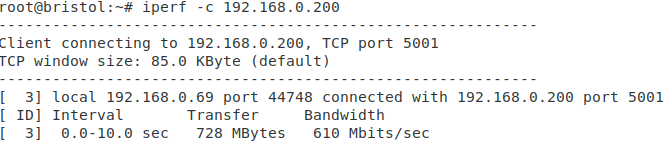
\includegraphics[width=14cm]{figures/q3-1-1.png}
\centering
\caption{Cos - TCP Iperf}
\centering
\label{fig:throughput_scenario_3}
\end{figure}


\begin{figure}[H]
\centering
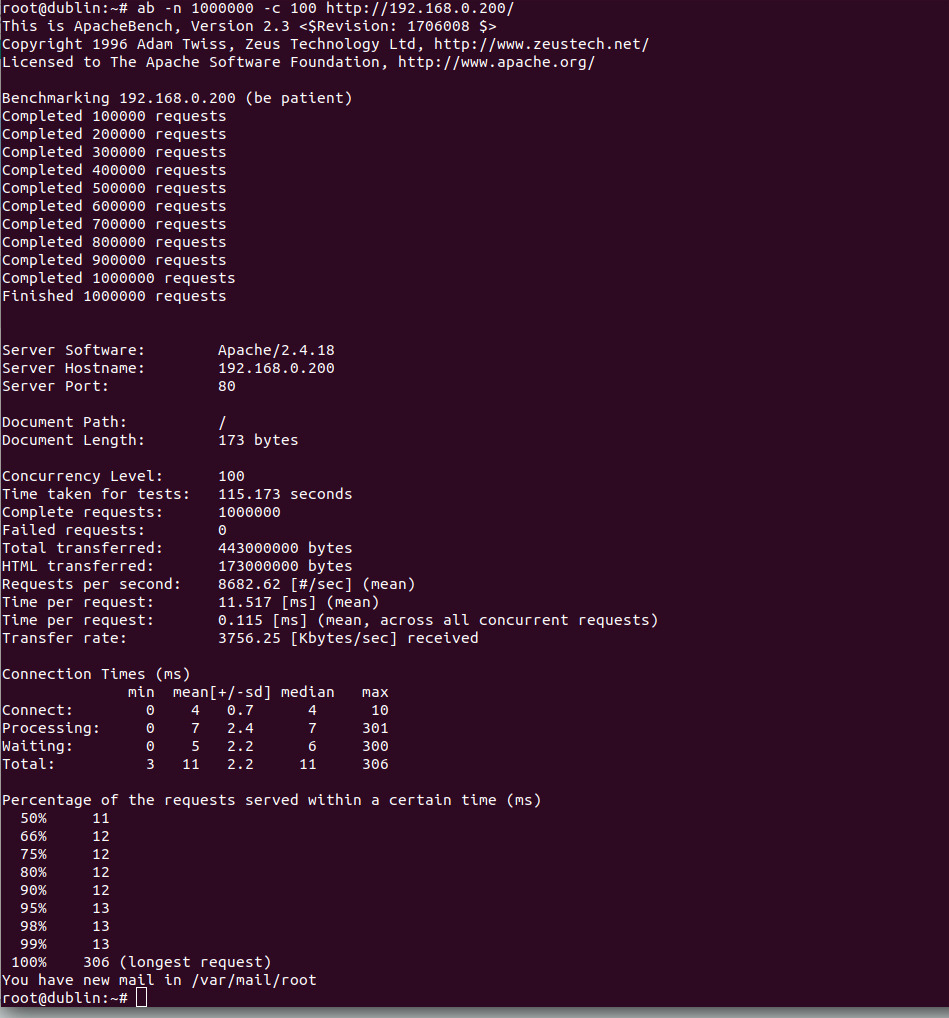
\includegraphics[width=14cm]{figures/dublin-ab2.png}
\caption{Cos - Apache Benchmark from Dublin client to Apache server with CoS enabled}
\centering
\label{fig:ab2_dublin_scenario_3}
\end{figure}


\begin{figure}[H]
\centering
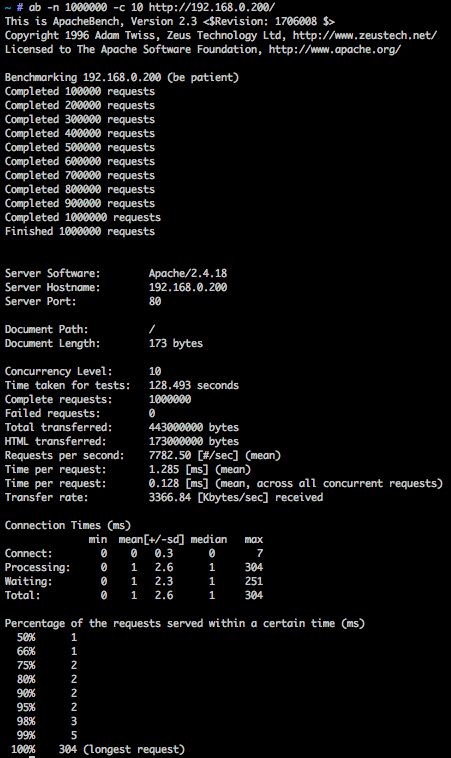
\includegraphics[width=12cm]{figures/calais-ab2.png}
\caption{Cos - Apache Benchmark from client to Apache server with CoS enabled}
\centering
\label{fig:ab2_calais_scenario_3}
\end{figure}

Now the TCP-transfer through \texttt{iperf} has much more bandwidth allocated, meaning the prioritisation of the ports appears to work. In order to confirm the results, this test was run twice.

\subsubsection{Difference between SRR shape and share}
Configuration for shape:
\begin{verbatim}
    conf t
    int G1/0/19
    srr-queue bandwidth shape 9830 9830 9830 9830
    int G1/0/17
    srr-queue bandwidth shape 9830 9830 9830 9830
    int G1/0/23
    srr-queue bandwidth shape 45000 45000 45000 45000
\end{verbatim}

Configuration for share:
\begin{verbatim}
    conf t
    int G1/0/19
    srr-queue bandwidth share 15 15 15 15
    int G1/0/17
    srr-queue bandwidth share 15 15 15 15
    int G1/0/23
    srr-queue bandwidth share 70 70 70 70
\end{verbatim}

\begin{figure}[H]
\centering
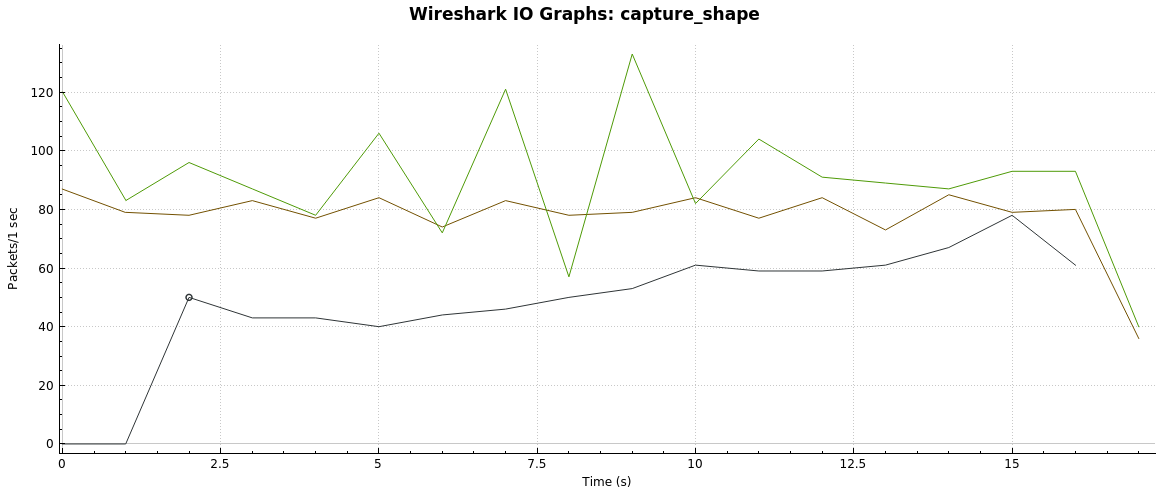
\includegraphics[width=14cm]{figures/screenshots_shape.png}
\caption{Packets per second sent after shape configuration}
\centering
\label{fig:shape_result}
\end{figure}

\begin{figure}[H]
\centering
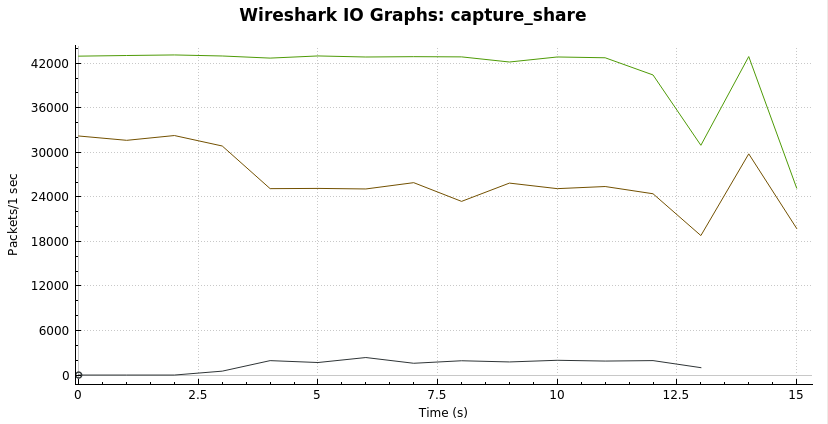
\includegraphics[width=14cm]{figures/screenshots_share.png}
\caption{Packets per second sent after share configuration}
\centering
\label{fig:share_result}
\end{figure}

Given the fact that the framesize of the \texttt{iperf} traffic (darkest line) varies from 5858 to 40610 bytes and the framesize of the HTTP-traffic (other two lines) vary from 66 to 147 bytes, the results shown in \textit{Figures \ref{fig:shape_result} and \ref{fig:share_result}} are correct. Both images show the packets sent per second, which should, according to the configured share and shape, result in a higher throughput for the \texttt{iperf} traffic. The throughput can be calculated using $Throughput_{traffic} = Packets/s_{traffic} * Frame size$ for every point per traffic type. As the size of the frames for the \texttt{iperf} traffic is much higher, the throughput is also higher which displays the queue share and shape values being applied. 

Comparing both figures (\ref{fig:share_result} and \ref{fig:shape_result}, the difference between sharing and shaping is displayed. With shaping, the throughput is limited to a configured value. With sharing, the traffic gets a guaranteed share of a queue, but is not limited to a value when extra bandwidth is available. We can see this based on the increase in \textit{Figure \ref{fig:share_result}}, when the \texttt{iperf} traffic line decreases. In \textit{Figure \ref{fig:shape_result}} we see the amount of packets sent per second bumping into a limit and then bouncing back. The value does not become higher than the limit.

\subsection{Q4.1 Mark your outgoing packets using iptables}
One of the characteristics of DSCP is that the classification of the packets can occur at the source (sender of specific traffic). The marking of the packets can be done using iptables, which is simply separating them into classes based on the protocol or ports used.\\
\\
The rule we have configured is for HTTP traffic (We run it on port 5000):

\begin{verbatim}
sudo iptables -t mangle -A OUTPUT -p tcp --dport 5000 -j DSCP --set-dscp-class cs3
\end{verbatim}

The result of the following command shows the value set in the DSCP field:
\begin{verbatim}
    iptables -t mangle -L -v
\end{verbatim}

The result is:
\begin{verbatim}
    Chain OUTPUT (policy ACCEPT 1217 packets, 202K bytes)
 pkts bytes target     prot opt in     out     source               destination         
    1    40 DSCP       tcp  --  any    any     anywhere             anywhere        \    
    tcp dpt:5000 DSCP set 0x18
\end{verbatim}

So, in the next question we would see HTTP traffic in our tcpdump to be marked with 0x18. In Wireshark the ToS-value is shown. According to https://www.tucny.com/Home/dscp-tos, the ToS value for DSCP 0x18 is 0x60.

\subsection{Q4.2 Show that the packets are marked}
In order to show the packets are marked, a \texttt{tcpdump} was started on one of the servers. The resulting PCAP-file was analysed using Wireshark. To check whether DSCP was applied to packets, we searched through the packets using filter \texttt{ip.dsfield.dscp}. The DSCP-value was retrieved from the \texttt{Differentiated Services Field} and is shown in \textit{Figure \ref{fig:dscp_marker}}. 

\begin{figure}[H]
\centering
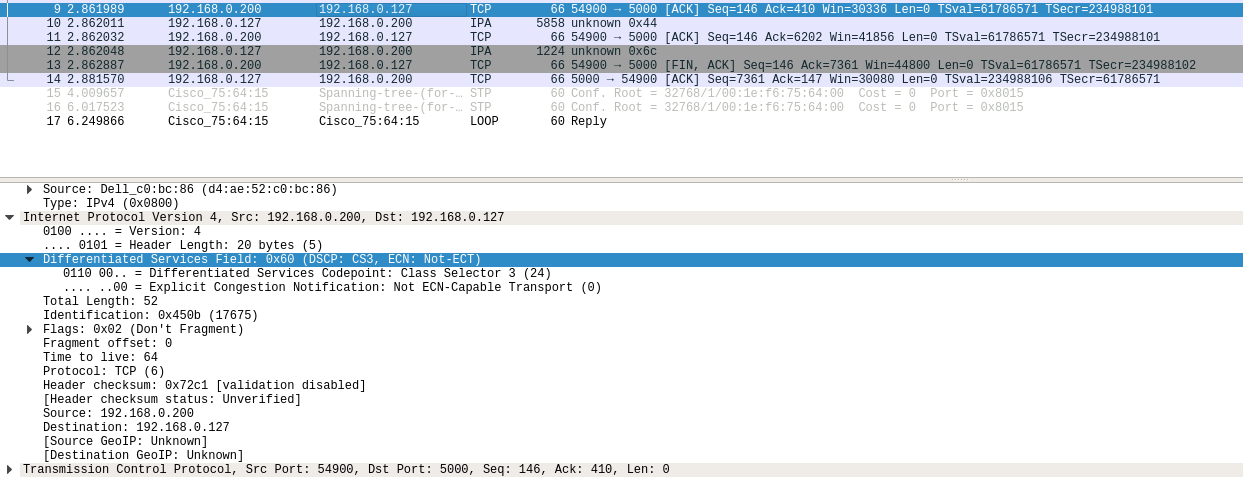
\includegraphics[width=17cm]{figures/dscp_marker.png}
\caption{DSCP marker 0x18 (ToS: 0x60)}
\centering
\label{fig:dscp_marker}
\end{figure}

\subsection{Q4.3 Show how DSCP marking improves traffic performance.}
In order to allow DSCP marking, we configured all ports of the switch to trust DSCP markings on ports. We did this using command:
\begin{verbatim}
    mls qos trust dscp
\end{verbatim}

We also configured the default DSCP-CoS mapping:
\begin{verbatim}
    mls qos map cos-dscp 10 15 20 25 30 35 40 45
\end{verbatim}

The results of the baseline tests are shown in \textit{Figures \ref{fig:ad_no-dscp} and \ref{fig:iperf_no-dscp}}. The figures show the bandwidth share between an \texttt{iperf} connection and an HTTP-connection. The \texttt{iperf} connection appears to be much faster. However, after configuring DSCP we did not see much improvement (only 2 Mbps in the \textttt{iperf} traffic). This is shown in \textit{Figures \ref{fig:ab_dscp} and \ref{fig:iperf_dscp}}.


\begin{figure}[H]
\centering
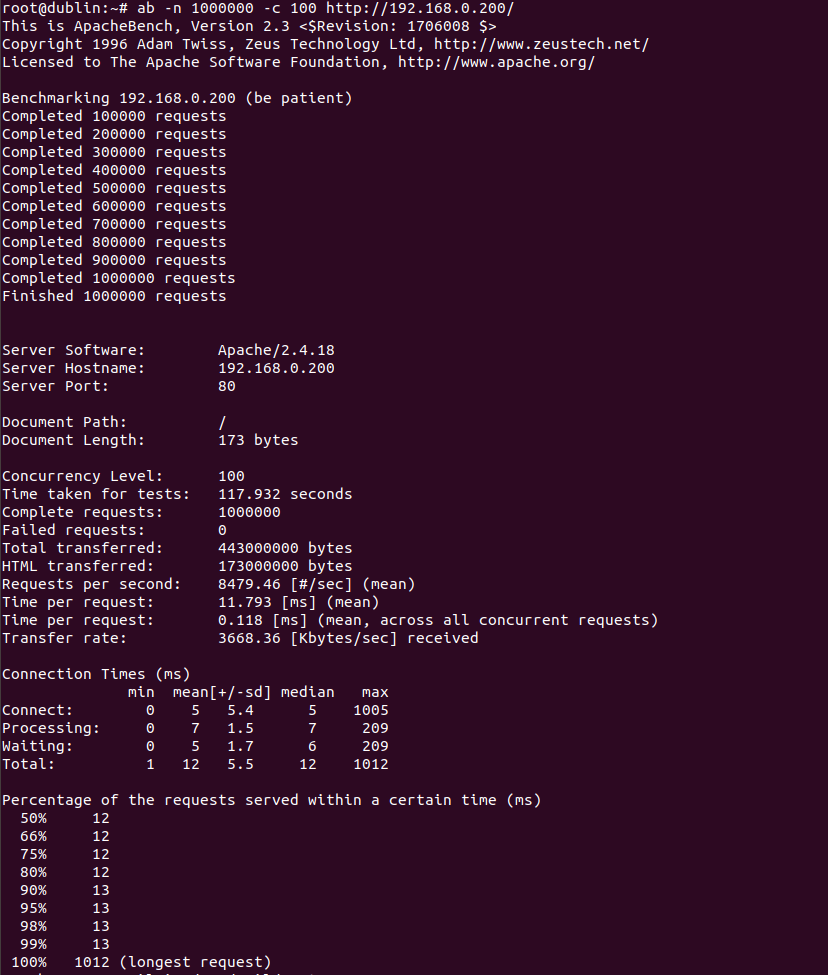
\includegraphics[width=15cm]{figures/q4-3-ab-no-dscp.png}
\caption{AB without DSCP enabled}
\centering
\label{fig:ad_no-dscp}
\end{figure}


\begin{figure}[H]
\centering
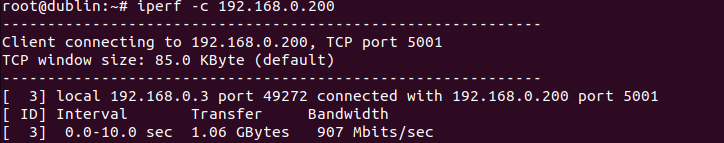
\includegraphics[width=15cm]{figures/q4-3-iperf-no-dscp.png}
\caption{iperf without DSCP enabled}
\centering
\label{fig:iperf_no-dscp}
\end{figure}


\begin{figure}[H]
\centering
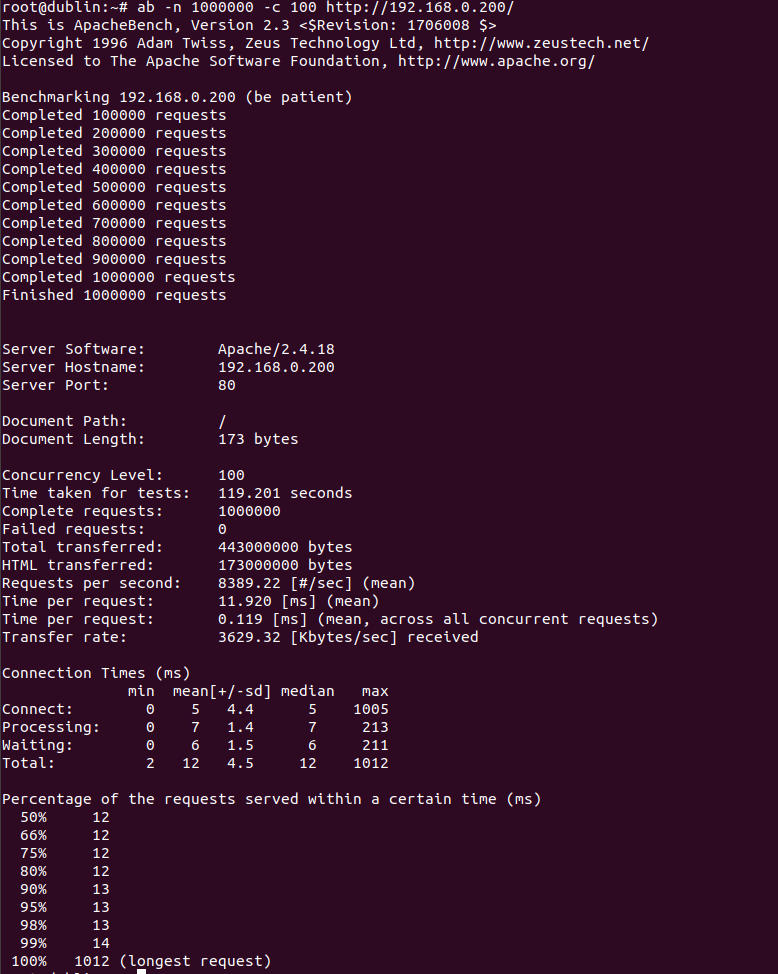
\includegraphics[width=15cm]{figures/q4-3-ab-dscp.png}
\caption{AB with DSCP enabled}
\centering
\label{fig:ab_dscp}
\end{figure}


\begin{figure}[H]
\centering
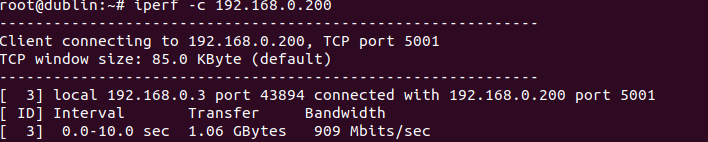
\includegraphics[width=15cm]{figures/q4-3-iperf-dscp.png}
\caption{iperf with DSCP enabled}
\centering
\label{fig:iperf_dscp}
\end{figure}








\subsection{Q5.1 Enable logging of events (syslog) to an external server.}

By default, syslog is enabled on cisco switches by default. We just need to forward the log to our server. The following command will do that:

\begin{verbatim}
gr3switch(config)#logging host 192.168.0.69
gr3switch(config)#snmp-server enable traps syslog

Follow the procedure given by this website to \textit{configure remote logging}:
https://du5tin.com/2017/06/10/set-up-syslog-server-in-ubuntu-server-16-04-w-log-rotation/

/var/log # tail -n2 /var/log/remote/192.168.0.253/syslog.log                                                                                                             root@calais
2018-02-22T18:03:56.342718+01:00 192.168.0.253 183: *Mar  3 05:03:57.338: %SYS-5-CONFIG_I: Configured from console by henrilarose on vty0 (192.168.0.127)
2018-02-22T18:04:42.496568+01:00 192.168.0.253 184: *Mar  3 05:04:43.550: %SYS-5-CONFIG_I: Configured from console by henrilarose on vty0 (192.168.0.127)
\end{verbatim}

\subsection{Q5.2 Monitor your switch so that its statistics can be viewed online. This requires to poll via
SNMP.}

We chose for monitoring NetDisco.

Following the installation process of the Perl/Postgres/Netdisco Stack is fairly simple following Netdisco's instructions.

https://metacpan.org/pod/App::Netdisco

\begin{verbatim}
    netdisco@calais:~\$ ~/bin/netdisco-backend start
Netdisco Backend                                              [Started]
config watcher: watching /home/netdisco/environments for updates.
\end{verbatim}

\begin{figure}[H]
\centering
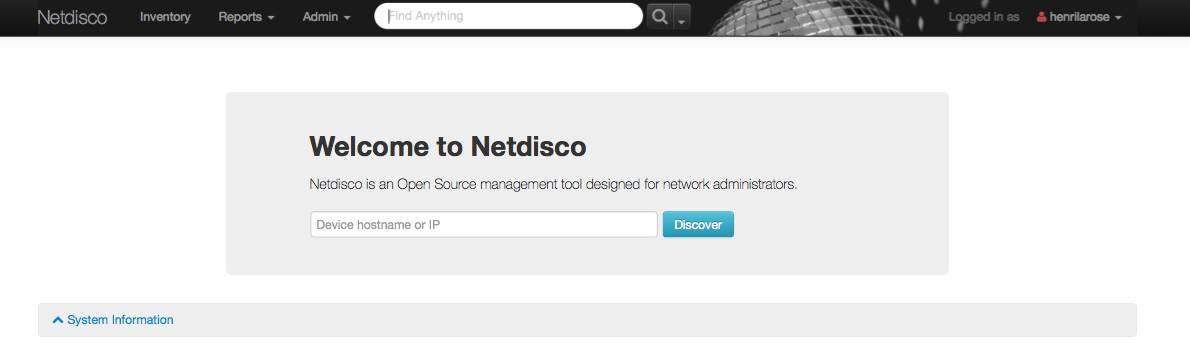
\includegraphics[width=17cm]{figures/screenshot_netdisco.png}
\caption{Netdisco network manager Web-Server}
\centering
\label{fig:dscp_marker}
\end{figure}

However, we can't figure out how to make the web-server receive the SNMP syslog traps from the switch. Thus, Netdisco cannot discover the devices on the server.

Switch SNMP configurations:
\begin{verbatim}
    snmp-server community an-cos RO
snmp-server community public RO
snmp-server community private RW
snmp-server location os3
snmp-server contact henrilarose
snmp-server enable traps syslog
snmp-server host 192.168.0.127 an-cos  snmp
snmp-server host 192.168.0.127 henrilarose  syslog
\end{verbatim}

Switch SNMP status:
\begin{verbatim}
    gr3switch#sh snmp
Chassis: FOC1151Z7ZQ
Contact: henrilarose
Location: os3
4122 SNMP packets input
    0 Bad SNMP version errors
    0 Unknown community name
    0 Illegal operation for community name supplied
    0 Encoding errors
    4115 Number of requested variables
    0 Number of altered variables
    0 Get-request PDUs
    4115 Get-next PDUs
    0 Set-request PDUs
    0 Input queue packet drops (Maximum queue size 1000)
4122 SNMP packets output
    0 Too big errors (Maximum packet size 1500)
    0 No such name errors
    0 Bad values errors
    0 General errors
    4115 Response PDUs
    0 Trap PDUs
SNMP global trap: disabled

SNMP logging: enabled
    Logging to 192.168.0.127.162, 0/10, 0 sent, 0 dropped.
SNMP agent enabled
\end{verbatim}

After an email exchange with Paola, \textit{snmpwalk}, on the server which runs Netdisco, was able to find all devices:
\begin{verbatim}
    iso.3.6.1.2.1.1.1.0 = STRING: "Cisco IOS Software, C3750 Software (C3750-IPSERVICESK9-M), Version 12.2(55)SE10, RELEASE SOFTWARE (fc2)
Technical Support: http://www.cisco.com/techsupport
Copyright (c) 1986-2015 by Cisco Systems, Inc.
Compiled Wed 11-Feb-15 11:40 by prod_rel_team"
iso.3.6.1.2.1.1.2.0 = OID: iso.3.6.1.4.1.9.1.516
iso.3.6.1.2.1.1.3.0 = Timeticks: (20331806) 2 days, 8:28:38.06
iso.3.6.1.2.1.1.4.0 = ""
iso.3.6.1.2.1.1.5.0 = STRING: "gr3switch.gr3.com"
iso.3.6.1.2.1.1.6.0 = ""
iso.3.6.1.2.1.1.7.0 = INTEGER: 6
iso.3.6.1.2.1.1.8.0 = Timeticks: (0) 0:00:00.00
...
iso.3.6.1.2.1.4.22.1.3.1.192.168.0.3 = IpAddress: 192.168.0.3
iso.3.6.1.2.1.4.22.1.3.1.192.168.0.69 = IpAddress: 192.168.0.69
iso.3.6.1.2.1.4.22.1.3.1.192.168.0.127 = IpAddress: 192.168.0.127
iso.3.6.1.2.1.4.22.1.3.1.192.168.0.200 = IpAddress: 192.168.0.200
iso.3.6.1.2.1.4.22.1.3.1.192.168.0.253 = IpAddress: 192.168.0.253
...
\end{verbatim}

However, the Netdisco back-end server does not seem to be able to do that. We were not able to configure it with Ralph either.



\end{document}


